% Main document
\documentclass[11pt,a4paper]{report}
%\documentclass[openany]{report}
% Section numbering without chapter prefix
\renewcommand{\thesection}{\arabic{section}}

% Roman numerals
\newcommand{\RNum}[1]{\uppercase\expandafter{\romannumeral #1\relax}}


% Required packages
\usepackage{mathptmx}
\usepackage[most]{tcolorbox}
\usepackage[utf8]{inputenc}
\usepackage[T1]{fontenc}
\usepackage{graphicx}
\usepackage{tabularx}
\usepackage{xltabular}
\usepackage{float}
\usepackage{amsmath}
\usepackage{amssymb}
\usepackage[style=apa,backend=biber]{biblatex}
\usepackage{hyperref}
\hypersetup{hidelinks, colorlinks=false}
\usepackage{cleveref}
\usepackage{lipsum}
\usepackage{eso-pic}
\usepackage{transparent}
\usepackage{xcolor}

%\usepackage{titlesec}

%\titlespacing*{\chapter}{0pt}{0pt}{20pt}

% Bibliography file
\addbibresource{references.bib}

% Document settings
\setlength{\parindent}{1em}
\setlength{\parskip}{1em}
\setcounter{tocdepth}{1}

% Page numbering (roman)
\pagenumbering{roman}

% set colors inverted for dev 
\definecolor{mydark}{HTML}{1F1F1F}
%\pagecolor{mydark}
%\color{white}


\begin{document}

% Front matter
\begin{titlepage}

%\AddToShipoutPictureBG*{%
%    \put(59.5,480){% Adjust these coordinates
%        \parbox[b]{0.8\paperwidth}{%
%            \centering
%            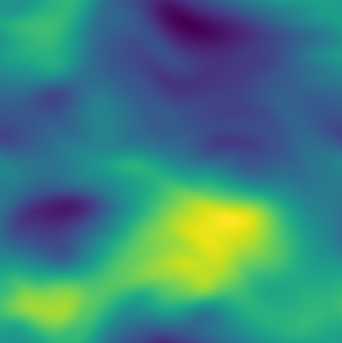
\includegraphics[width=0.66\linewidth]{misc./fluidGPT.png}%
%        }%
%    }%
%}
    \begin{center}
        \vspace*{2cm}

        \LARGE
        \bf FluidGPT: Highly-dimensional Foundation Modelling for Navier Stokes
        
        \large Deterministic vs Probabilistic \\ stable sequencing
        \vspace{4cm}

        \large
        Tom Harmsen \\
        Supervision: Vlado Menkovski

        \vfill

        \normalsize
        Draft Report\\[0.3cm]
        For the degree of MSc Data Science \& Artificial Intelligence\\
        Department of Mathematics and Computer Science\\
        University of Technology Eindhoven\\[2cm]

        June 2026

    \end{center}
\end{titlepage}
%\input{frontmatter/declaration}
%\input{frontmatter/acknowledgements}
%\input{frontmatter/summary}

% Table of contents and lists
%\tableofcontents
%\clearpage
%\listoftables
%\clearpage
%\listoffigures
%\clearpage

% Page numbering (arabic)
\pagenumbering{arabic}

% Main chapters
\chapter{Introduction}\label{ch:introduction}

\section{Motivation}

Fluid dynamics governs a vast range of physical phenomena, from atmospheric circulation and ocean currents to industrial flow systems and aerodynamic design. At the heart of many of these processes lies the Navier-Stokes system of partial differential equations, which describes the conservation of mass and momentum in a fluid medium. Despite their well-established theoretical foundation, the Navier-Stokes equations remain notoriously difficult to solve in practice. Their nonlinear, coupled structure gives rise to complex multi-scale behaviour that often requires high-resolution numerical methods and substantial computational resources. As a result, large-scale simulation campaigns can become prohibitively expensive, particularly when many trajectories must be evaluated repeatedly for design, optimisation, or scientific analysis.

Recent advances in machine learning have created new opportunities to accelerate fluid simulation through the use of \emph{surrogate models}. Rather than solving the governing equations directly, a surrogate learns to predict future system states from previously observed states, transfering the cost of simulation into a training phase and enabling orders-of-magnitude faster inference. Such models have demonstrated promising results on individual fluid dynamics benchmarks and increasingly complex flow regimes.

However, many existing surrogate models are developed and evaluated within relatively narrow settings, often focusing on a single dataset, flow configuration, or physical regime. Real-world fluid dynamics encompasses a much broader spectrum of behaviours, including laminar and turbulent flows, compressible and incompressible dynamics, diverse boundary conditions. Understanding whether a single neural architecture can learn effectively across this heterogeneous landscape is therefore an important step toward more generally applicable fluid dynamics surrogate model.

\section{Problem Statement}

Building a foundation model for Navier-Stokes dynamics presents several fundamental challenges. First, the governing system exhibits qualitatively different behaviour depending on the flow regime. Laminar and turbulent flows, compressible and incompressible conditions, forced and unforced dynamics, and diverse boundary geometries each impose distinct structural constraints on the solution manifold. A model trained on a narrow subset of these conditions will generalise poorly to others, making breadth of training data a critical prerequisite.

Second, turbulent fluid dynamics are intrinsically stochastic in character at the macroscopic level. Even though the Navier-Stokes equations are deterministic, extreme sensitivity to initial conditions means that small errors in the initial state can rapidly propagate into qualitatively different trajectories. A deterministic surrogate model, constrained to produce a single point estimate of the future state, may therefore be fundamentally ill-suited to capture this distributional uncertainty. A probabilistic formulation that learns a conditional distribution over plausible futures is a natural alternative, but imposes its own challenges in terms of architecture design, training stability, and sampling efficiency.

Third, accurate long-horizon prediction requires not only low single-step error but also that predictions remain physically consistent over many autoregressive steps. Error accumulation during rollout is a well-documented failure mode of data-driven surrogate models, and mitigating it demands both architectural choices that promote temporal stability and training procedures that are robust to distributional shift between teacher-forced training and free-running inference.

\section{Approach}

This work addresses these challenges through a comparative study of two surrogate modelling approaches for two-dimensional Navier-Stokes dynamics, trained jointly on a heterogeneous multi-source dataset spanning nine distinct flow configurations.

Both approaches share a common hierarchical backbone, combining a Swin Transformer \citep{Liu2021SwinTA} with a factorised space-then-time attention mechanism embedded in a UNet-style encoder-decoder architecture. This design enables efficient multi-scale feature extraction across spatial and temporal dimensions, with skip connections preserving fine-grained information across resolution levels. The backbone is adapted from the standard image-classification Swin Transformer to handle sequential, spatiotemporal input and to return predictions at the original spatial resolution.

The two modelling strategies differ in their prediction formulation. The \textbf{deterministic model} directly maps a block of five historical velocity field states to the subsequent five states, minimising a mean-squared error objective. The \textbf{probabilistic model} adopts a flow-matching formulation \citep{Lipman2022FlowMatching}, learning to transport samples from a structured Gaussian prior to the target distribution of future states conditioned on the same historical input. By sampling from the prior at inference time, the probabilistic model produces a distribution of plausible futures rather than a single prediction, offering a principled way to represent the inherent uncertainty of turbulent dynamics.

The pre-training dataset is assembled from nine datatsets, covering compressible and incompressible flows, laminar and turbulent regimes, periodic and Dirichlet boundary conditions, and a wide range of initialisation schemes. Together, the datasets contribute approximately 21 TB of simulated two-dimensional velocity field trajectories.

\section{Contributions}

The main contributions of this work are as follows:

\begin{enumerate}
    \item \textbf{A custom spatiotemporal backbone for fluid dynamics.} We design and implement a hierarchical Swin Transformer backbone extended with factorised space-then-time attention blocks and a UNet-style encoder-decoder structure, specifically adapted for multi-dataset pretraining on two-dimensional Navier-Stokes velocity fields.

    \item \textbf{A probabilistic flow-matching surrogate model.} We develop and train a conditional flow-matching model that learns a distribution over future fluid states, conditioned on historical velocity inputs. The model employs a structured spatially-correlated Gaussian prior and integrates over flow-time using a fixed-step Euler scheme, and is shown to outperform deterministic baselines on the large majority of evaluated datasets.

    \item \textbf{Large-scale multi-source pretraining.} We curate, preprocess, and unify nine heterogeneous datasets into a common training pipeline, covering a broad spectrum of Navier-Stokes regimes and providing a foundation for generalisation across flow conditions.

    \item \textbf{Systematic evaluation across accuracy, stability, and spectral fidelity.} We evaluate both model families under single-step, autoregressive rollout, and spectral diagnostics settings, providing a structured comparison of deterministic and probabilistic modelling strategies for fluid dynamics.
\end{enumerate}

\section{Report Structure}

The remainder of this report is organised as follows. Chapter~\ref{ch:problem} formally defines the Navier-Stokes system, the machine learning objective, and the dual modelling framework. Chapter~\ref{ch:datasets} describes the nine pretraining datasets and the preprocessing pipeline. Chapter~\ref{ch:models} details the shared backbone architecture, the mathematical formulation of the attention mechanisms, and the specific design of the deterministic and flow-matching model variants. Chapter~\ref{ch:training} describes the training framework, hardware platform, optimisation strategy, and validation methodology. Chapter~\ref{ch:results} presents and discusses the experimental results across single-step prediction, autoregressive rollout, and spectral analysis.
\chapter{Problem Formulation}

This chapter formally defines the research problem, establishing the specific physical PDE system, the constraints imposed by large-scale pretraining data, and the mathematical framework for the two proposed AI surrogate models. We further detail the key challenges that motivate the dual deterministic-probabilistic modelling approach, before concluding with the research questions guiding this work.

\section{Navier-Stokes System}

The Navier–Stokes equations describe the dynamics of fluid flow through a set of coupled, nonlinear partial differential equations that enforce conservation of both mass and momentum. In this work, we focus on the two-dimensional, isothermal case, governed by the following equations:

\begin{gather}\label{eq:navierstokes}
\partial_t \rho + \nabla \cdot (\rho \mathbf{u}) = 0, \\
\partial_t \mathbf{u} + (\mathbf{u} \cdot \nabla) \mathbf{u} = -\frac{1}{\rho} \nabla p + \frac{1}{\rho} \nabla \cdot \boldsymbol{\tau} + \mathbf{f}, \\
B_i(\mathbf{u}, p)|_{\partial \Omega} = g_i, \quad \mathbf{u}(0) = A, \quad x \in \Omega=[0,1]^2.
\end{gather}

Here, $\rho$ denotes density, $\mathbf{u}$ the velocity vector field, $p$ the pressure, $\boldsymbol{\tau}$ the viscous stress tensor, and $\mathbf{f}$ an external forcing term. The first equation expresses conservation of mass (continuity), while the second represents momentum conservation. Boundary and initial conditions are specified by $B_i$ and $A$, respectively.

In the special case of incompressible flow, the simplification $\frac{d\rho}{dt} = 0$ is applied, which reduces the complexity of the operator's input–output mapping. This enforces no stretching and compressing of the fluid, also referred to as divergence-free flow.

\vspace{1em}

\subsection{Characteristics of the Navier–Stokes System}\label{sec:energyspectra}

The Navier–Stokes system shows complex dynamical behavior characterized by creation, advection, and dissipation of vortical structures, often referred to as eddies. Large eddies break down into smaller eddies in a cascading process, transferring energy across lowering scales until it dissipates at the smallest (viscous) level. This process is chaotic and highly sensitive to initial conditions, leading to stochastic-like macroscopic behavior even though the governing equations are deterministic. Capturing this behavior accurately is a core challenge for surrogate models, especially those that must generalize across varying flow regimes and boundary conditions.

\vspace{1em}

\textbf{Energy and Enstrophy Spectra.}
To quantify the cascade process of energy and vorticity across scales, the flow field is often analyzed in Fourier space. The energy spectrum $E(k)$ characterizes the distribution of kinetic energy among different wavenumbers $k$, describing how much energy is contained in eddies of their respective scale. It is defined as
\begin{equation}
	E(k) = \frac{1}{2} \int_{|\mathbf{k}| = k} |\hat{\mathbf{u}}(\mathbf{k})|^2 \, d\mathbf{k},
\end{equation}
where $\hat{\mathbf{u}}(\mathbf{k})$ denotes the Fourier transform of the velocity field. In turbulence modelling, when energy is transferred from the larger eddies to the smaller eddies, then a \textit{direct energy cascade} is inferred, for which a schematic example can be viewed in Figure \ref{fig:energyspectrumscheme}. Alternatively, when energy flows in the opposite direction, the flow is referred to as an \textit{inverse energy cascade}. For turbulent divergence-free Navier-Stokes flows, the typical Kolmogorov scaling law is defined by $E(k) \sim k^{-5/3}$ within the inertial subrange \citep{Kolmogorov1941}.

\begin{figure}[H]
	\centering
	\includegraphics[width=0.8\textwidth]{figs/turbulence_scales2.png}
	\caption{Schematic of typical energy cascade process of Navier-Stokes governed system. Energy is injected at highest wavenumbers and dissipated at lowest wavenumbers. Energy is transferred in sequential manner across the scales in between, referred to as the inertial subrange. Note that most of the energy in the system is contained in the larger size vortices.}
	\label{fig:energyspectrumscheme}
\end{figure}

Similarly, the enstrophy spectrum $Z(k)$ describes the spectral distribution of vorticity magnitude, reflecting the rotational activity of the flow across scales. It is defined as
\begin{equation}
	Z(k) = \frac{1}{2} \int_{|\mathbf{k}| = k} |\hat{\boldsymbol{\omega}}(\mathbf{k})|^2 \, d\mathbf{k},
\end{equation}
where $\boldsymbol{\omega} = \nabla \times \mathbf{u}$ is the vorticity field. For turbulent divergence-free flows, the typical Kolmogorov scaling law is defined by $Z(k) \sim k^{-3}$ within the inertial subrange \citep{Kolmogorov1941}.

\section{Pre-training Datasets and Preliminary Domain Coverage}\label{se:datasetconditions}

To enable the model to generalise across the full range of Navier–Stokes regimes, a diverse ensemble of 2-dimensional pre-training datasets is needed. The Navier–Stokes equation exhibits a broad spectrum of behaviour depending on flow type (laminar or turbulent), compressibility, boundary conditions, and external forcing. Capturing these variations requires data originating from multiple numerical solvers, simulation conditions, and initialisation schemes. For our datasets we seek uniform grid simulated data.

We aim to select datasets with coverage of the following type:
\begin{enumerate}
	\item Compressible and incompressible simulations
	\item Laminar and turbulent flow regimes
	\item Different boundary conditions
	\item With and without forcing terms
	\item Distinct initialisation methods
	\item Parameter variations in viscosity, pressure, and density
\end{enumerate}

Collectively, the coverage ensures that the pre-training process exposes the model to a broad spectrum of physical behaviours. A detailed description of each dataset, including its generation method, resolution, and specific parameters, will be provided in the methodology section.

\section{Machine Learning Objective}

The objective of this work is to construct a model $\mathcal{M}$ that predicts the future evolution of a continuous-time, partial differential equation (PDE) system, specifically the Navier-Stokes equations, across a wide and diverse parameter space.

The system state is defined by the flow variable $\mathbf{u}(\mathbf{x}, t)$, which is the 2D velocity field:
\begin{equation*}
\mathbf{u}(\mathbf{x}, t) = [u_x(\mathbf{x}, t), u_y(\mathbf{x}, t)]^T,
\end{equation*}
where $u_x$ and $u_y$ are the velocity components in the $x$ and $y$ directions, respectively, in a spatial domain $\Omega \subset \mathbb{R}^2$ at time $t$. The governing physics are implicitly defined by the Navier-Stokes equations, which can be summarized in the general form:

\begin{equation}
	\frac{\partial \mathbf{u}}{\partial t} + \mathcal{F}(\mathbf{u}, \nabla \mathbf{u}, \nabla^2 \mathbf{u}; \mathbf{c}) = 0 \quad \text{in } \Omega \times (0, \infty)
\end{equation}

with appropriate initial conditions and boundary conditions. The vector $\mathbf{c} \in \mathcal{C}$ denotes a set of system parameters (Reynolds number $Re$, domain geometry, and boundary conditions, etc.) that condition the flow.

\subsection{Prediction Task}

In the context of a discrete-time, data-driven surrogate model, the spatial domain $\Omega$ is discretized into a grid, $\mathbf{x} \in \Omega_h$ with resolution $128^2$. The system state at a time step $t_i$ is represented by a high-dimensional tensor $\mathbf{U}_i \in \mathbb{R}^{N_x \times N_y \times 2}$, where $N_x, N_y$ are the number of grid points in the spatial dimensions, and $2$ represents the input flow variables ($u_x$ and $u_y$).

Given an input sequence of $\Delta T > 1$ historical flow states:
\begin{equation*}
\mathbf{S}_{\text{in}} = \{ \mathbf{U}_{T_0-\Delta T}, \mathbf{U}_{T_0-\Delta T+1}, \ldots, \mathbf{U}_{T_0-1} \},
\end{equation*}
the core prediction problem is to model the evolution operator $\mathcal{P}_{\mathbf{c}}$ such that the model $\mathcal{M}$ accurately predicts the subsequent $\Delta T$ future states:
\begin{equation*}
\mathbf{S}_{\text{out}} = \{ \mathbf{U}_{T_0}, \mathbf{U}_{T_0+1}, \ldots, \mathbf{U}_{T_0+\Delta T-1} \}.
\end{equation*}
The model $\mathcal{M}$ is a function of the input sequence $\mathbf{S}_{\text{in}}$ and the system parameter vector $\mathbf{c}$.
\begin{equation*}
\mathcal{M}(\mathbf{S}_{\text{in}}) \approx \mathcal{P}_{\mathbf{c}}(\mathbf{S}_{\text{in}})
\end{equation*}

\section{Dual Modelling Approach}

This problem is tackled using two distinct modeling approaches, which define the specific mathematical targets of the prediction. Both models now condition their output on a sequence of the $k$ most recent past states, $\mathbf{S}_{\text{in}}$, and are trained to predict a bundle of $\Delta T$ future states, $\mathbf{S}_{\text{pred}}$.

\subsection{1. Deterministic Prediction}
This approach models the conditional expectation of a short-sequence bundle of five future states, $\mathbb{E}[\mathbf{S}_{\text{out}} | \mathbf{S}_{\text{in}}]$. It utilizes a function $f_{\theta}$ that maps the historical sequence to the predicted future sequence:
\begin{equation*}
f_{\theta}: \mathbf{S}_{\text{in}} \mapsto \mathbf{S}_{\text{out}}
\end{equation*}
The predicted sequence of states is:
\begin{equation*}
\hat{\mathbf{S}}_{\text{out}} = f_{\theta}(\mathbf{S}_{\text{in}}).
\end{equation*}
For long rollouts, the prediction system is auto-regressive: the predicted sequence $\hat{\mathbf{S}}_{\text{out}}$ is sequentially reused as the new input $\mathbf{S}_{\text{hist}}$ to predict the next $\Delta T$ steps.

The learning objective for the model parameters $\theta$ is the minimization of a mean-squared error (MSE) loss $\mathcal{L}_{\text{AR}}$, measuring the error over the entire predicted sequence bundle:
\begin{equation*}
\mathcal{L}_{\text{AR}}(\theta) = \mathbb{E}_{(\mathbf{S}_{\text{in}}, \mathbf{S}_{\text{out}}) \sim \mathcal{D}} \left[ \| \mathbf{S}_{\text{out}} - f_{\theta}(\mathbf{S}_{\text{in}}) \|_2^2 \right].
\end{equation*}

\subsection{2. Probabilistic Prediction (Flow Matching)}
Given the possible turbulent nature of the system, the evolution over a long horizon $T$ is better described by the transition of a probability distribution $p(\mathbf{U}_{T_0+T} | \mathbf{S}_{\text{in}})$ rather than a deterministic one.

The goal is to train a model $\mathcal{M}_{\phi}$ with parameters $\phi$ that effectively models this conditional probability distribution:
\begin{equation*}
\mathcal{M}_{\phi}(\mathbf{S}_{\text{in}}) \approx p( \mathbf{S}_{\text{out}} | \mathbf{S}_{\text{in}}).
\end{equation*}
\textbf{Flow Matching} achieves this by learning the velocity field $\mathbf{v}_{\phi}(\mathbf{z}, \tau)$ that transforms a simple prior distribution (like Gaussian noise) into the complex target distribution $p$ via a continuous-time ordinary differential equation (ODE) trajectory: $\frac{d\mathbf{z}}{d\tau} = \mathbf{v}_{\phi}(\mathbf{z}, \tau)$, where $\tau \in [0, 1]$ is an artificial time. By conditioning on the previous system states $\mathbf{S}_{\text{in}}$, the model can better identify the appropriate statistical flow regime, allowing it to efficiently sample from the manifold of physically plausible solutions and ensuring long-term temporal stability and statistical fidelity. Note that the velocity field and artificial time in this context are different definitions than the velocity field and time of the physical Navier-Stokes system.

Denote the loss term for the Flow Matching model as $\mathcal{L}_{\text{FM}}$. Following the conditional formulation, this objective measures how well the learned velocity field $\mathbf{v}_{\phi}(\mathbf{z}, \tau)$ approximates the target transport field $\tilde{\mathbf{v}}(\mathbf{z}, \tau)$, which defines the transformation between the source and target distributions along the artificial time dimension $\tau \in [0, 1]$. The training loss is defined as the mean-squared deviation between the predicted and target velocities:
\begin{equation*}
	\mathcal{L}_{\text{FM}}(\phi) = 
	\mathbb{E}_{\tau,\,(\mathbf{z}, \tilde{\mathbf{v}}) \sim \mathcal{D}} 
	\left[
	\big\| 
	\mathbf{v}_{\phi}(\mathbf{z}, \tau \mid \mathbf{S}_{\text{in}}) 
	- 
	\tilde{\mathbf{v}}(\mathbf{z}, \tau)
	\big\|_2^2
	\right].
\end{equation*}

\section{Challenges}\label{sec:challenges}

Building a foundation surrogate model for Navier-Stokes dynamics that is accurate, stable, and broadly applicable across heterogeneous flow regimes presents several fundamental challenges. These challenges, several of which were introduced briefly in the problem statement of Chapter~\ref{ch:introduction}, are elaborated here in the context of the formal modelling framework established above. They jointly motivate the dual deterministic-probabilistic approach and the evaluation strategy adopted in this work.

\subsection{Heterogeneity of the Flow Regime Space}

As formalised in Section~\ref{se:datasetconditions}, the system parameter vector $\mathbf{c} \in \mathcal{C}$ spans a wide and structurally diverse space: laminar versus turbulent regimes, compressible versus incompressible dynamics, forced versus unforced systems, and a range of boundary conditions and initialisation schemes. Each of these axes imposes qualitatively different constraints on the solution manifold of $\mathcal{P}_{\mathbf{c}}$. For instance, incompressible flows are constrained to the divergence-free subspace of velocity fields, whereas compressible flows permit local density variation and admit shock-like discontinuities absent from the incompressible regime. Forcing terms $\mathbf{f}$ introduce sustained energy injection that can drive a system toward a statistically stationary turbulent state, while unforced systems instead exhibit monotonic decay of kinetic energy over time.

A single neural operator $\mathcal{M}$ trained naively across this combined space risks learning an averaged representation that fails to capture regime-specific structure, particularly when the relative sampling frequency of each regime in the combined training corpus $\mathcal{D}$ is imbalanced. This raises an architectural and data-curation challenge: the model must be expressive and conditioned enough to disambiguate between regimes from the historical input $\mathbf{S}_{\text{hist}}$ alone, without explicit access to the ground-truth parameter vector $\mathbf{c}$ at inference time.

\subsection{Sensitivity to Initial Conditions and the Limits of Deterministic Prediction}

As discussed in Section~\ref{sec:energyspectra}, the Navier-Stokes system exhibits highly chaotic dynamics within turbulent regimes. Despite being governed by deterministic equations, the underlying energy cascade rapidly amplifies infinitesimal perturbations across spatial and temporal scales, redistributing them through the creation, advection, and dissipation of vortical structures. Consequently, nearly identical historical states $\mathbf{S}_{\text{in}}$ can diverge into vastly different future trajectories $\mathbf{S}_{\text{out}}$ over a sufficiently long horizon $T$, with individual eddies decaying, merging, or shedding along distinct, individually plausible paths.

This divergence exposes a major failure mode in the deterministic formulation $f_\theta$ introduced in Section 3.4.1, which inherently targets the conditional expectation $\mathbb{E}[\mathbf{S}_{\text{out}} \mid \mathbf{S}_{\text{in}}]$. When the true conditional distribution $p(\mathbf{S}_{\text{out}} \mid \mathbf{S}_{\text{in}})$ admits several such plausible vortex-decay paths, the deterministic model responds by averaging across all of them pointwise in physical space. Because the position, phase, and strength of a decaying eddy generally differ from one plausible path to the next, this average does not correspond to any single coherent vortex structure; it instead washes out the sharp, high-frequency features of the flow, yielding an over-smoothed, low-energy state that represents a statistical blend rather than a physically realisable trajectory, and ultimately fails to satisfy the governing conservation laws at any individual time step.

To circumvent this averaging artefact, a predictive model must instead possess a natural, built-in capacity to represent the full space of plausible vortex evolutions, and to sample a single coherent realisation from it, rather than collapsing them into one blended estimate. This requirement motivates the probabilistic flow-matching framework detailed in Section 3.4.2, which directly models the full conditional distribution $p(\mathbf{S}_{\text{out}} \mid \mathbf{S}_{\text{in}})$ rather than its mean. Each sample drawn from this distribution can follow one self-consistent vortex-decay path to completion, preserving the sharp gradients and kinetic energy of an individually realisable flow field, while the spread of the distribution itself naturally reflects how tightly or loosely the historical state $\mathbf{S}_{\text{in}}$ constrains the underlying decay process: where the dynamics are nearly deterministic, the learned distribution can collapse to a narrow, sharply peaked density around a single dominant path, and where genuine multi-modality exists, whether due to strong turbulence or a subtle bifurcation in an otherwise weakly perturbed flow, it can instead spread mass across several distinct outcomes. The model is therefore not forced to make an arbitrary singular choice in either regime, but instead inherits the same underlying flexibility, expressed only to the degree that the data demands it.

\subsection{Long-Horizon Autoregressive Stability}

Both modelling approaches rely on autoregressive rollout to extend predictions beyond the directly trained horizon $\Delta T$: the predicted sequence $\hat{\mathbf{S}}_{\text{out}}$ is fed back as the new historical input $\mathbf{S}_{\text{hist}}$ for the next prediction step. This introduces a well-documented failure mode in data-driven PDE surrogates, namely the compounding of small per-step errors over many rollout iterations. Because the model is trained under teacher forcing on ground-truth trajectories from $\mathcal{D}$, but evaluated at inference time on its own previously generated (and therefore imperfect) outputs, a distributional shift between training and inference conditions emerges. In systems with the sensitivity properties described above, this shift can be amplified rather than damped, leading to rapid divergence, unphysical artefacts, or loss of high-wavenumber spectral content over long rollouts. Mitigating this requires both architectural inductive biases that promote stability, such as the multi-scale, factorised attention structure of the shared backbone, and training procedures that better expose the model to its own distribution of inference-time errors.

\subsection{Physical Consistency Beyond Pointwise Accuracy}

Pointwise error metrics, such as the mean-squared error underlying $\mathcal{L}_{\text{AR}}$, do not necessarily capture whether a prediction is physically plausible. A prediction can achieve low pointwise error while still violating expected statistical properties of turbulent flow, for instance by failing to reproduce the Kolmogorov scaling laws of the energy and enstrophy spectra introduced in Section~\ref{sec:energyspectra}, or by exhibiting unphysical energy injection or excessive numerical dissipation across the inertial subrange. This is a particular risk for autoregressive rollouts, where high-wavenumber content is often the first to degrade. Evaluating surrogate models therefore requires spectral diagnostics in addition to pointwise accuracy metrics, in order to assess whether predictions remain consistent with the underlying physics of the energy cascade, rather than merely close to the ground truth in an aggregate sense.

\subsection{Multi-Source Data Heterogeneity and Normalisation}

Beyond the physical heterogeneity discussed above, the nine datasets selected for pretraining (Section~\ref{se:datasetconditions}) originate from distinct numerical solvers, each with its own discretisation scheme, native resolution, temporal sampling rate, and units. Unifying this data into the common tensor representation $\mathbf{U}_i \in \mathbb{R}^{N_x \times N_y \times 2}$ at a shared resolution of $128^2$ requires consistent resampling, normalisation, and temporal alignment strategies. Inconsistent normalisation across datasets with markedly different characteristic velocity or energy scales risks biasing the training loss toward higher-magnitude datasets, while overly aggressive normalisation risks erasing physically meaningful scale information, such as the effective Reynolds number, that the model would otherwise need to infer from the input sequence alone.

\section{Research Questions}

This work focuses on building a foundation model that is both rollout-stable and physically consistent for a wide domain space of Navier–Stokes flows, relying solely on velocity-field inputs. To tackle this, we take a dual approach, leveraging deterministic and probabilistic modeling techniques. The following research questions highlight the objectives of our study, each directly motivated by the challenges outlined in Section~\ref{sec:challenges}.

\begin{enumerate}
	\item \textbf{Can probabilistic flow matching models outperform deterministic baselines in predicting subsequent system states of Navier-Stokes dynamics, when trained on a heterogeneous multi-source dataset spanning a wide variety of physical parameters and flow regimes?}
	\item \textbf{How does autoregressive rollout error accumulate over time for probabilistic versus deterministic models, and does the probabilistic formulation confer greater long-horizon stability across datasets of varying temporal length?}
	\item \textbf{Do the predicted system states satisfy physical characteristics as measured by spectral analysis, and do probabilistic models produce spectrally more consistent predictions than deterministic models across flow regimes?}
\end{enumerate}

%\input{chapters/chapter1/chapter1}
%\input{chapters/chapter2/chapter2}
%\input{chapters/chapter3/chapter3}
%\input{chapters/chapter4/chapter4}
% Bibliography
\begin{sloppypar}
    \printbibliography[heading=bibintoc,title=References]
\end{sloppypar}

% Appendices
\appendix
% Main appendix file that includes all other appendices
\appendix
\section{Additional Material}
%\label{app:appendices}

% Include individual appendix files
%\input{appendices/appendix_chapter2}
%\input{appendices/appendix_chapter3}

\end{document}
